\documentclass[a4paper,11pt]{article}
\usepackage{amsmath,amsthm,amsfonts,amssymb,amscd,amstext,vmargin,graphics,graphicx,tabularx,multicol} 
\usepackage[francais]{babel}
\usepackage[utf8]{inputenc}  
\usepackage[T1]{fontenc} 
\usepackage{pstricks-add,tikz,tkz-tab,variations}
\usepackage[autolanguage,np]{numprint} 

\setmarginsrb{1.5cm}{0.5cm}{1cm}{0.5cm}{0cm}{0cm}{0cm}{0cm} %Gauche, haut, droite, haut
\newcounter{numexo}
\newcommand{\exo}[1]{\stepcounter{numexo}\noindent{\bf Exercice~\thenumexo} : \marginpar{\hfill /#1}}
\reversemarginpar


\newcounter{enumtabi}
\newcounter{enumtaba}
\newcommand{\q}{\stepcounter{enumtabi} \theenumtabi.  }
\newcommand{\qa}{\stepcounter{enumtaba} (\alph{enumtaba}) }
\newcommand{\initq}{\setcounter{enumtabi}{0}}
\newcommand{\initqa}{\setcounter{enumtaba}{0}}

\newcommand{\be}{\begin{enumerate}}
\newcommand{\ee}{\end{enumerate}}
\newcommand{\bi}{\begin{itemize}}
\newcommand{\ei}{\end{itemize}}
\newcommand{\bp}{\begin{pspicture*}}
\newcommand{\ep}{\end{pspicture*}}
\newcommand{\bt}{\begin{tabular}}
\newcommand{\et}{\end{tabular}}
\renewcommand{\tabularxcolumn}[1]{>{\centering}m{#1}} %(colonne m{} centrée, au lieu de p par défault) 
\newcommand{\tnl}{\tabularnewline}

\newcommand{\trait}{\noindent \rule{\linewidth}{0.2mm}}
\newcommand{\hs}[1]{\hspace{#1}}
\newcommand{\vs}[1]{\vspace{#1}}

\newcommand{\N}{\mathbb{N}}
\newcommand{\Z}{\mathbb{Z}}
\newcommand{\R}{\mathbb{R}}
\newcommand{\C}{\mathbb{C}}
\newcommand{\Dcal}{\mathcal{D}}
\newcommand{\Ccal}{\mathcal{C}}
\newcommand{\mc}{\mathcal}

\newcommand{\vect}[1]{\overrightarrow{#1}}
\newcommand{\ds}{\displaystyle}
\newcommand{\eq}{\quad \Leftrightarrow \quad}
\newcommand{\vecti}{\vec{\imath}}
\newcommand{\vectj}{\vec{\jmath}}
\newcommand{\Oij}{(O;\vec{\imath}, \vec{\jmath})}
\newcommand{\OIJ}{(O;I,J)}


\newcommand{\bmul}[1]{\begin{multicols}{#1}}
\newcommand{\emul}{\end{multicols}}

\newcommand{\reponse}[1][1]{%
\multido{}{#1}{\makebox[\linewidth]{\rule[0pt]{0pt}{20pt}\dotfill}
}}

\newcommand{\titre}[5] 
% #1: titre #2: haut gauche #3: bas gauche #4: haut droite #5: bas droite
{
\noindent #2 \hfill #4 \\
#3 \hfill #5

\vspace{-1.6cm}

\begin{center}\rule{6cm}{0.5mm}\end{center}
\vspace{0.2cm}
\begin{center}{\large{\textbf{#1}}}\end{center}
\begin{center}\rule{6cm}{0.5mm}\end{center}
}



\begin{document}
\pagestyle{empty}
\titre{Interrogation : Cosinus d'un angle}{Nom :}{Prénom :}{Classe}{Date}



\exo{3,5}

\q Pour chaque question, mettre la lettre correspondant à la bonne réponse dans la dernière case.

\begin{flushleft}
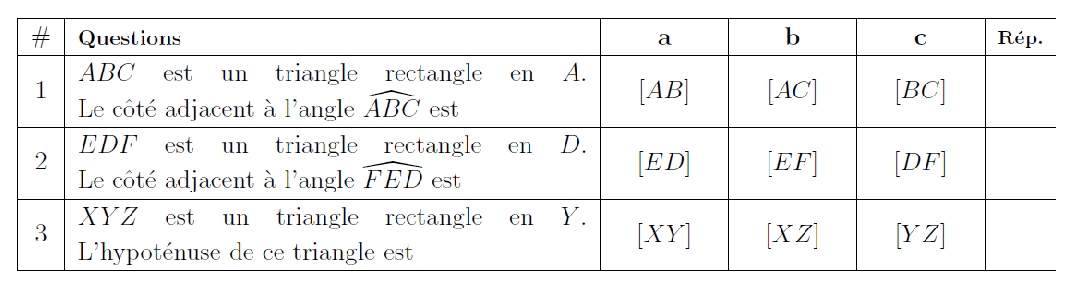
\includegraphics[scale=1]{qcm.eps} 
\end{flushleft}



\q Compléter le tableau suivant : \\

\begin{tabular}{|c|c|c|c|c|}
\hline 
Mesure de l'angle (arrondi au degré) & 31 &  & 68 &  \\ 
\hline 
Cosinus de l'angle (arrondi au millième) &  & 0,675 &  & 0,117 \\ 
\hline 
\end{tabular} 

\vspace*{1cm}

\exo{2}

\initq \q Soit EFG un triangle rectangle en E tel que : $\widehat{EGF}$ = 45 et FG = 4 cm.\\

Calculer EG. (Donner la valeur approchée au dixième près)

\noindent \reponse[5]\\


\q Soit LEA un triangle rectangle en A tel que :$\widehat{ELA}$ = 68 et LA = 7 cm.\\


Calculer LE. (Donner la valeur approchée au dixième près)

\noindent \reponse[5]\\

\exo{2,5}

On considère le triangle TRI tel que : IR=14,4cm ; IT = 27cm et TR = 30,6 cm.\\


\initq \q Démontrer que le triangle TRI est un triangle rectangle.\\
\reponse[5]\\

\newpage

\q Calculer la mesure, en degré, de chacun des angles aigus du triangle TRI. On donnera les arrondis au dixième.\\
\reponse[5]\\

\exo{2,5}

On considère la figure ci-dessous, dans laquelle les points A,O, D d'une part, B, O, C d'autre part, sont alignés.\\

\begin{center}
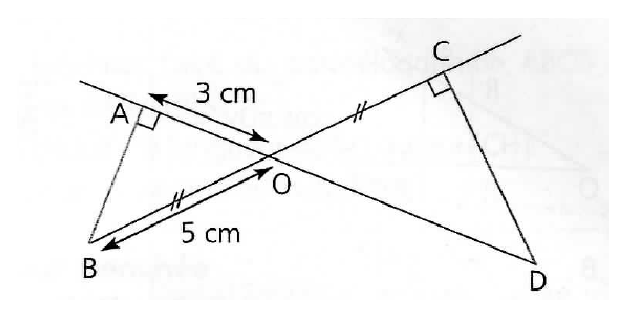
\includegraphics[scale=1]{fig.eps} 
\end{center}

\initq \q Calculer la mesure, en degré, de l'angle $\widehat{AOB}$.
En déduire la mesure, en degré, de l'angle $\widehat{COD}$. On donnera les arrondis au dixième.\\
\reponse[5]\\

\q Calculer OD. On donnera l'arrondi au mm.\\
\reponse[5]\\





\end{document}
